\chapter{Einleitung}

Zeitliche Veränderung in der Thematik von Texten zu erfassen ist eine wesentliche Aufgabe in der modernen, durch eine Flut von Informationen charakterisierten Gesellschaft. Dies kann von der Überwachung von Nachrichtentexten \citep{newsTopic} über Trenderkennung in Blogs \citep{blogpulse} bis zur Identifikation von Themen in Chats reichen. Die Anwendungen sind vielfältig. Im Kontext einer Lernplattform kann man sich einen Chat vorstellen, in dem Schüler sich über verschiedene zu bearbeitende Themen unterhalten. Ein Lehrer, der beobachtet über welche Themen gesprochen wird, könnte erkennen, ob erstens überhaupt etwas getan wird und zweitens, ob noch Lernbedarf besteht.

Die bisherigen Verfahren weisen oft Einschränkungen bei der Erkennung der Themen bzw. der Verifizierbarkeit der Themen auf. Oftmals müssen die Texte manuell annotiert werden, um die Themen erkennen zu können, oder die Themen sind nur aufwändig zu ermitteln \citep{ldaSourceCode}. Ferner ist die betrachtete Zeitspanne häufig nicht variabel genug bzw. wird bei der Erstellung des Modells zum Erkennen der Themen festgelegt und kann somit nicht unabhängig von den Themen betrachtet werden \citep{topicsOverTime}.

In dieser Diplomarbeit soll eine Methode entwickelt werden, um die zeitliche Änderung der Themen in Texten zu erfassen. Die einzelnen Textfragmente dieser sequentiellen Texte müssen eine zeitliche Ordnung aufweisen und somit sequentiell angeordnet werden können. Diese zu entwickelnde Methode soll eine möglichst große Variabilität bzgl. der betrachteten Zeitspanne bieten. Ergänzend soll der Aufwand in der Erkennung der thematischen Verläufe gering gehalten werden, so dass eine Online-Anwendung möglich ist. Um dies zu erreichen, wird folgende Methode vorgeschlagen.

Ausgehend von der Annahme, dass sequentielle Texte vorliegen, werden zuerst die Themen anhand Hintergrundwissen oder der vorliegenden Textkollektion gelernt. Anhand dieses Modells werden für die sequentiellen Texte die Themen bestimmt und eine relationale Struktur in Form eines Graphen aufgebaut. Auf diesen Graphen werden Zentralitätsmaße angewandt, um die Wichtigkeit der Themen numerisch zu erfassen. Die zeitlichen Verläufe der Zentralitätsmaße werden dann geeignet visualisiert. Da die Ergebnisse und die entwickelte Methode im EU-Projekt \textit{Science Created by You} (SCY) genutzt werden sollen, ergeben sich spezielle Anforderungen, die in Abschnitt \ref{chap:goals} noch genauer erläutert werden. 

Das SCY-Projekt\footnote{\href{http://www.scy-net.eu}{http://www.scy-net.eu}} ist ein EU-Projekt mit dem Ziel eine Plattform zu entwickeln, die es Schülern ermöglicht, selbstständig zu lernen. Im Gegensatz zu vielen anderen E-Learning Systemen bietet das SCY-Projekt eine Plattform, die kollaboratives Lernen verschiedener Inhalte unterstützt. Die Lerninhalte werden als Missionen modelliert, in denen den Schülern unterschiedliche Werkzeuge zur Verfügung stehen, um die gestellte Aufgabe zu lösen. 

Eine der ersten Missionen beschreibt die Aufgabe, ein \COTWO-neutrales Haus zu entwickeln. Dazu müssen die Schüler sich zuerst generell über \COTWO\  und dessen Auswirkung auf den Treibhauseffekt informieren. Anschließend informieren sie sich über Maßnahmen, die den \COTWO-Ausstoß eines Hauses senken können. Dies können verschiedene Baustoffe, Dämmmaterialien oder andere Techniken sein. Hierzu werden Hintergrundtexte gelesen und Simulationen  durchgeführt, die den Zusammenhang zwischen den verschiedenen \COTWO-Quellen und den Gegenmaßnahmen darstellen. Ausgehend von diesem Hintergrundwissen werden dann die Häuser entworfen. 

SCY unterstützt den Schüler dabei durch verschiedene Werkzeuge, die kollaborativ genutzt werden können. Insbesondere können sich die Schüler per Chat über etwaige Unklarheiten oder den Entwurf des Hauses austauschen. Die Chats werden aufgezeichnet und sollen als Quelle für die zu untersuchenden Textsequenzen dienen. Wie genau die Themenveränderungen in den Chat- und sonstigen Texten erfasst werden sollen, welche Schwierigkeiten dabei auftreten können und wie diese gelöst werden, wird in dieser Arbeit erläutert. 

\section{Ziele der Arbeit}
\label{chap:goals}


Das Ziel dieser Diplomarbeit ist es, die zeitliche Veränderung von Themen in Textsequenzen zu erfassen. Im Speziellen soll die Prominenz der Themen erfasst und die Veränderungen über die Zeit dargestellt werden. Ein Thema ist ein prominentes Thema, wenn es oft in einer Textsequenz auftritt. Es könnten nun, wie in es in \citet{ldaSourceCode} angewendet wird, für jeden Zeitabschnitt die Themen gelernt werden und gezählt werden, wie oft ein Thema vorkommt. Dieser Ansatz ist jedoch für die vorliegende Arbeit ungeeignet, da erstens die Ergebnisse als Online-Algorithmus im SCY-Projekt benutzt werden sollen und das Lernen der Themen doch eine zeitaufwändige Aufgabe ist. Zweitens werden hier die Wahrscheinlichkeiten des Auftretens der Themen nicht berücksichtigt, sondern es wird jedes Auftreten gezählt.

Der Ansatz in dieser Arbeit ist ähnlich, in wichtigen Punkten unterscheidet er sich jedoch. Zum einen wird zwischen der Lernphase und der Anwendungsphase unterschieden. In der Lernphase wird anhand von Hintergrundtexten ein Themenmodell trainiert. Diese Hintergrundtexte sind nicht notwendigerweise zeitlich sortiert und enthalten Informationen über die Themen, die trainiert werden sollen. Dies sind zum Beispiel Artikel der Deutschen Presse Agentur (dpa) zu bestimmten Themen wie Politik, Kunst oder, im Kontext des SCY-Projektes, Texte mit Hintergrundwissen für die aktuelle zu bearbeitende Mission. So kann ein Themenmodell erstellt werden, das für den speziellen Kontext geeignet ist. Diese Eignung soll in der Diplomarbeit auch validiert werden. Die genaue Vorgehensweise wird in Kapitel \ref{chap:workflowData} behandelt. Die Qualität der Themenmodelle hängt direkt von der Vorverarbeitung der Texte ab. Es muss also zusätzlich ermittelt werden, welche Vorverarbeitunsschritte die Qualität der Themenmodelle beeinflussen.

\begin{figure}[ht]
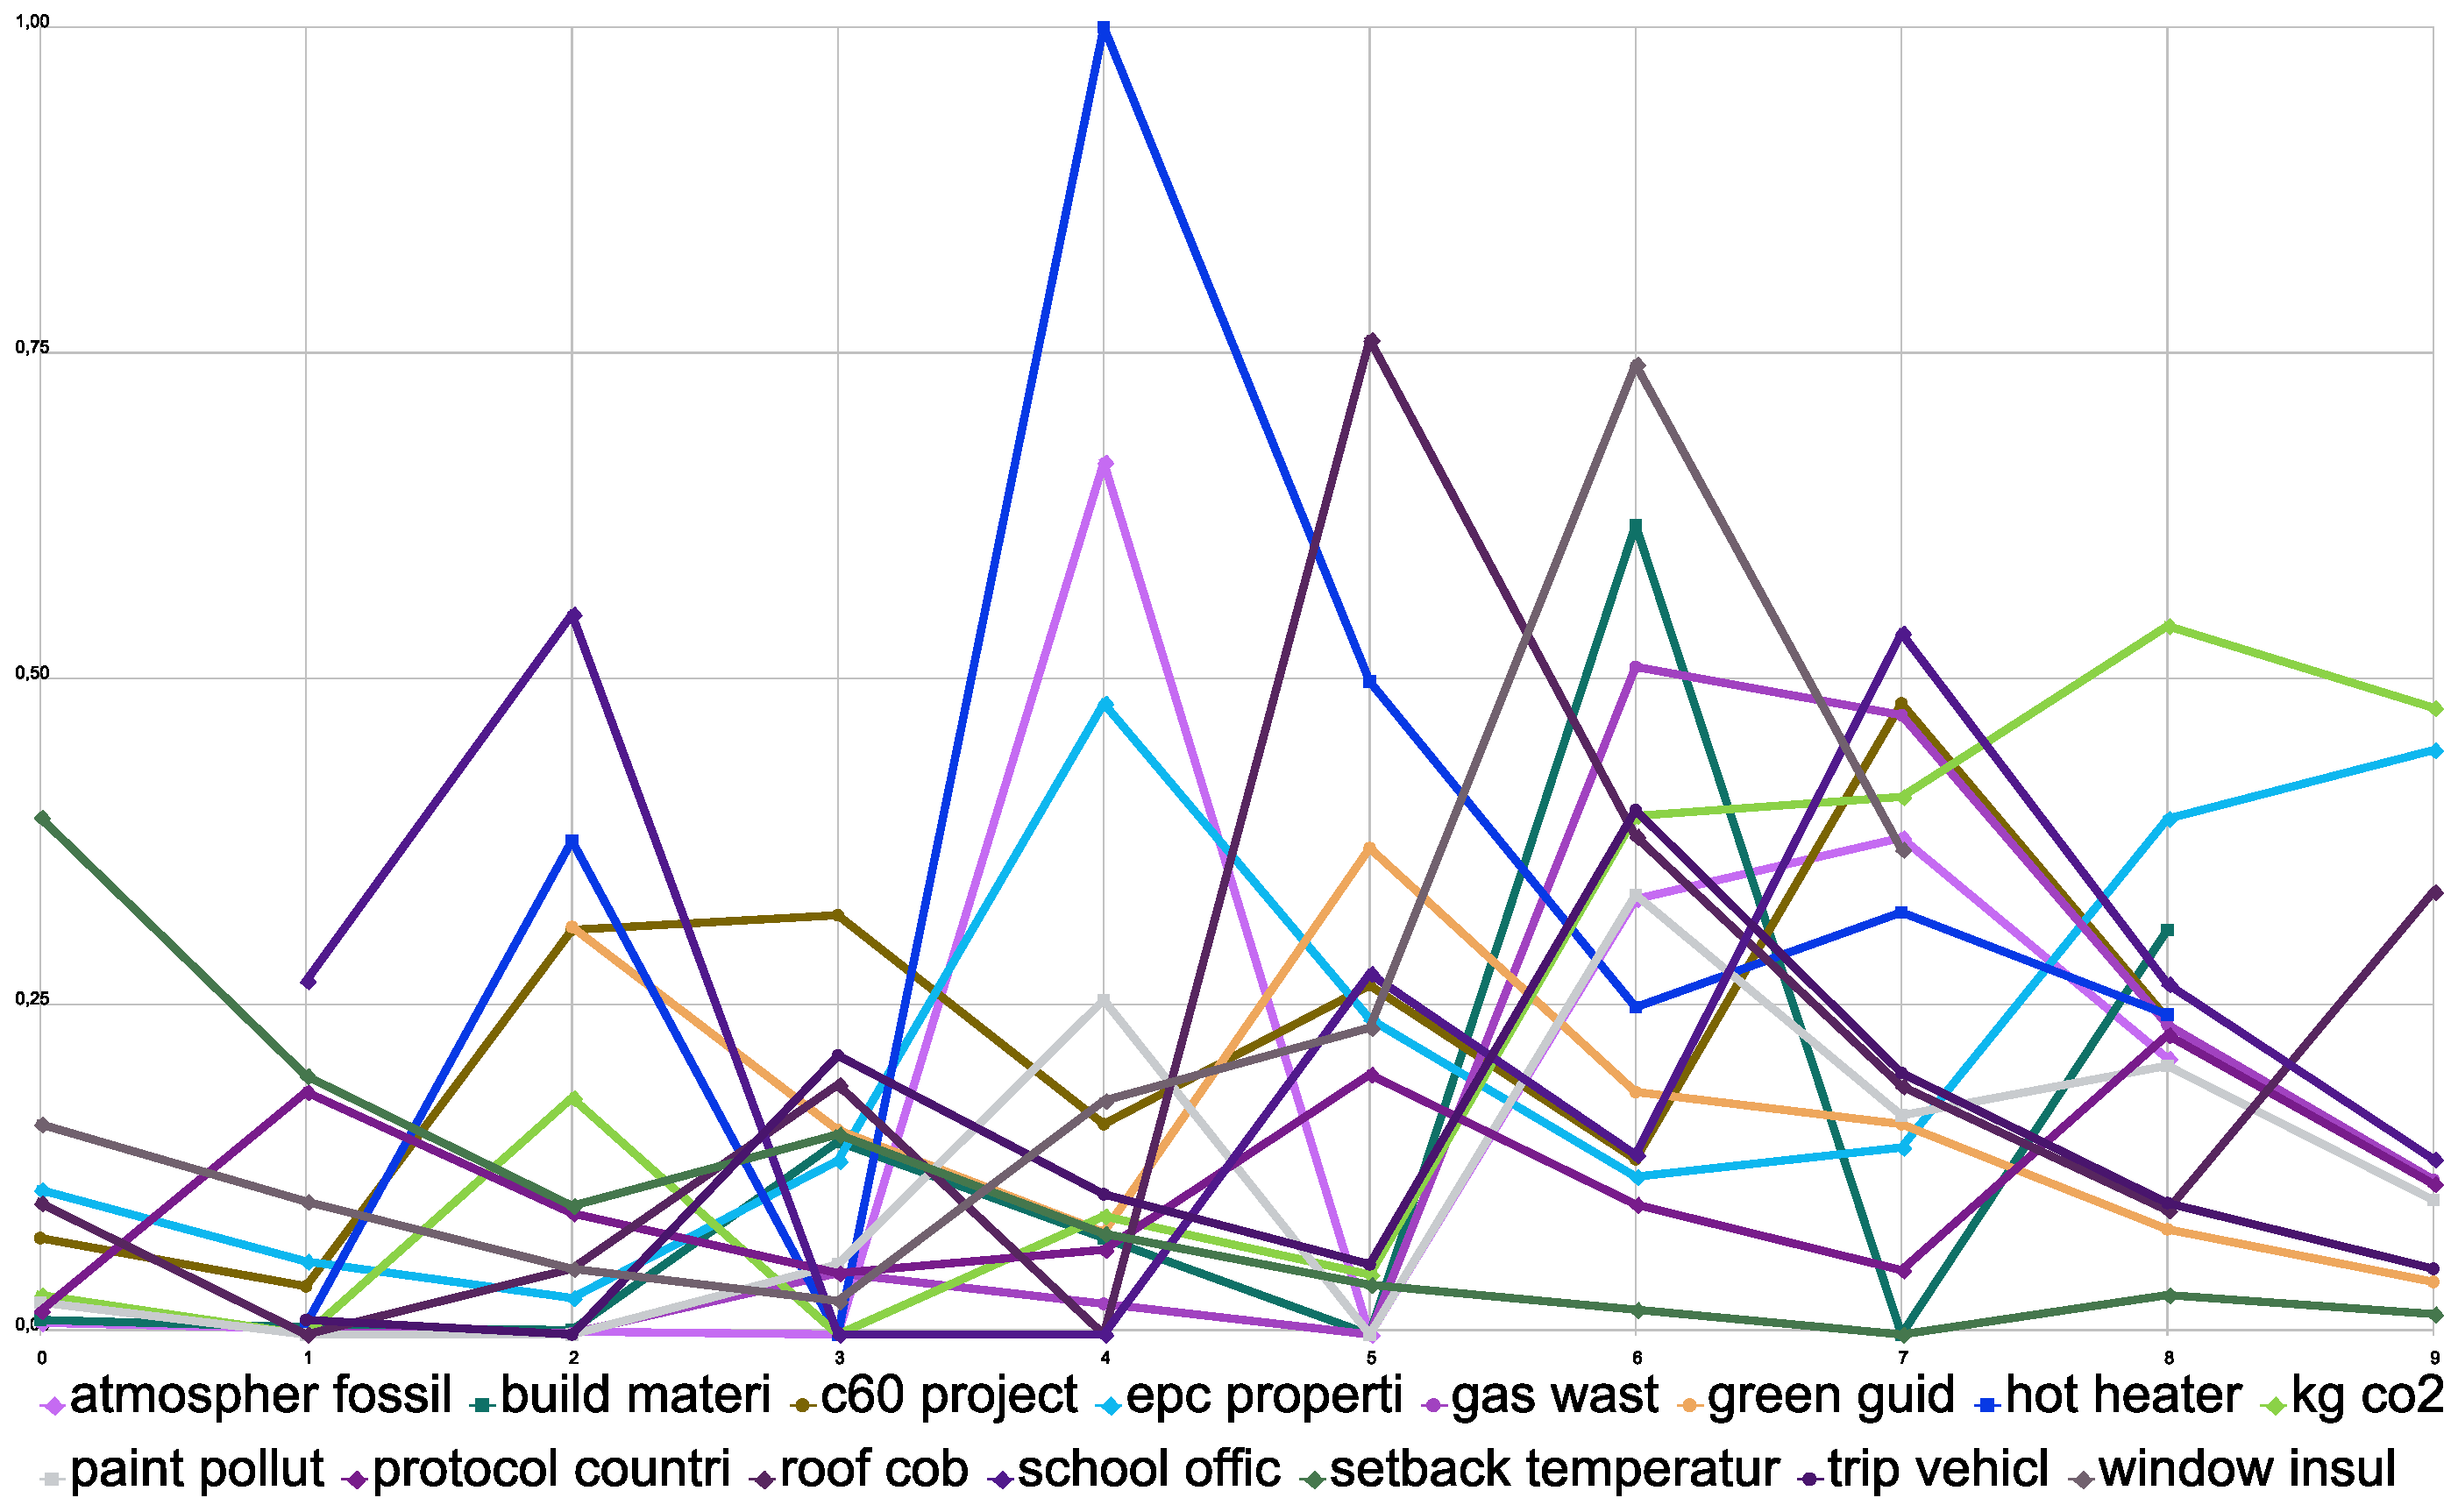
\includegraphics[width=1.0\textwidth]{images/content/01_introduction/chart_betweeness} 
\caption{Visualisierung der Themenveränderung}
\label{fig:topicChange}
\end{figure}

In der Anwendungsphase werden die vorkommenden Themen identifiziert, deren Wichtigkeit bewertet und schlussendlich die zeitliche Verände"-rung dargestellt. Dazu werden, wie in \citet{shafferEpistemicFrames}, die Textsequenzen in diskrete zeitliche Abschnitte unterteilt. Die Einteilung richtet sich dabei nach vorhandenen Dokumenten. In einen zeitlichen Abschnitt werden eine bestimmte Anzahl von zeitlich aufeinander folgenden Dokumenten zusammengefasst. Je nach Größe der Zeitabschnitte können so verschieden Zeiträume betrachtet werden. Im Falle von Chatnachrichten kann ein Zeitabschnitt nur ein paar Minuten umfassen, während im Falle von Nachrichten die Zeitabschnitte eine Woche, einen Monat oder mehr abdecken können. Da die Wahl der Größe der Zeitabschnitte unabhängig vom gelernten Themenmodell ist, können so auch verschiedene Zeiträume in annehmbarer Zeit betrachtet und verglichen werden. 

Für jedes Dokument in einem Zeitabschnitt werden die vorkommenden Themen und die Wahrscheinlichkeit, mit der diese Themen vorkommen, ermittelt. Aus den ermittelten Themen wird anhand der Kookkurrenz und den Wahrscheinlichkeiten eine Graphenstruktur aufgebaut. Es werden verschiedene Algorithmen entwickelt, die dann auf ihre Eignung geprüft werden. Auf die Graphen werden dann verschiedene Zentralitätsindizes angewendet. Zentralitätsindizes bewerten die Wichtigkeit eines Knoten in einem Graphen. So wird die Prominenz der Themen ermittelt. Auch hier gilt es zu evaluieren, welcher Zentralitätsindex am besten geeignet ist, die Prominenz der Themen zu bewerten. 

Wenn mehrere Zeitabschnitte nacheinander betrachtet werden, kann die thematische Verände"-rung einfach visualisiert werden. Hierzu werden die Veränderungen als Kurve dargestellt. In Abbildung \ref{fig:topicChange} ist ein Beispiel für eine solche Visualisierung dargestellt. Da die Visualisierung unübersichtlich werden kann, wenn viele Themen auftreten, werden auch hier verschiedene Ansätze untersucht.

Es gilt also folgende Probleme zu lösen: 
\begin{itemize} 
  \item Themenmodelle anhand von Hintergrundtexten zu trainieren und ihre Eignung für die Aufgabenstellung zu evaluieren.
  \item Textsequenzen in diskrete Zeitabschnitte zu unterteilen und festzustellen, welche Größe der Zeitabschnitte für die verschiedenen Textdatensätze geeignet ist.
  \item Aus den ermittelten Themen einen Graphen zu erstellen und zu prüfen, welcher Algorithmus zusammen mit den Zentralitätsindizes die zugrundeliegenden Themen in den Texten am besten repräsentiert.
  \item eine geeignet Art der Visualisierung entwickeln.
\end{itemize} 

\section{Zusammenfassung}
Im diesem Kapitel wurde die Motivation der geplanten Anwendung dargelegt und zwei Anwendungsbeispiele betrachtet. Anschließend wurde dargestellt, welche Ziele erreicht werden sollen und angeschnitten wie diese realisiert werden sollen. Dies wird in der weiteren Arbeit genauer beschrieben. 

In Kapitel \ref{chap:basics} wird auf die Grundlagen wie Themenmodelle und Zentralitätsmaße eingegangen, die in der Literatur schon erforscht wurden und hier nicht weiter entwickelt bzw. nur unverändert benutzt werden. Kapitel \ref{chap:relatedWork} stellt Arbeiten vor, die mit ähnlichen Ansätzen arbeiten, wie sie in der Diplomarbeit verfolgt werden. Das \ref{chap:workflowData}. Kapitel stellt die verwendeten Daten und die Vorarbeit, die für diese Daten nötig ist, dar. Insbesondere wird darauf eingegangen, welche Daten zum Training des Themenmodells benutzt und welche Daten als Textsequenz benutzt werden. 

Der eigentliche entwickelte Algorithmus, bzw. die Applikation zur Erkennung und Bewertung der Themen wird in Kapitel \ref{chap:workflowTime} erläutert. Dort werden die einzelnen Schritte dargestellt, wie man von einem sequentiellen Text zu einer Darstellung von thematischen Verläufen kommt. Zusätzlich werden Methoden zur Evaluation des Algorithmus entwickelt. Die Ergebnisse der durchgeführten Experimente und die Bewertung derselben wird in Kapitel \ref{chap:results} veranschaulicht. Im letzten Kapitel wird noch ein kurzer Ausblick auf verschiedene Anwendungen der entwickelten Methode gegeben und die Methode und ihre Ergebnisse kritisch hinterfragt. 



